%%% Stop the section counter from resetting when a new chapter is declared %%%
\makeatletter
  %\@removefromreset{section}{chapter}
\makeatother

\definecolor{myred}{rgb}{0.8, 0, 0} % Custom red colour

\geometry{a4paper,total={170mm,257mm},left=20mm,top=20mm,} % Custom margins

\renewcommand\contentsname{} % remove the "Chapter #" thing

\renewcommand{\thechapter}{\Roman{chapter}} % Change the dot point for chapters in Table of contents
\renewcommand{\thesection}{\arabic{section}} % Change the dot point for sections in table of contents 

\onehalfspacing % increase the spacing between the lines to something more readable / typical of a legal document

\clearpairofpagestyles % Clear all existing page styles to make way for our ones

%%% Lower the vertical margin so that the header doesn't feel as "squashed" %%%
\addtolength{\topmargin}{.35in}
\addtolength{\textheight}{-.45in}

%%% command to create the custom chapter headers %%%
\newcommand{\ChapterTitle}[2][]{\noindent
{\color{myred} \rule{\linewidth}{8.0mm}}\vspace{-7.6mm}\noindent
\textbf{ \color{white}\ \Large{#1 #2}}\vspace{6mm}
}

%%% command to create the custom section headers %%%
\newcommand{\SectionTitle}[2]{\noindent \hspace{6mm} {\xhrulefill{pink}{8.0mm}}

 \vspace{-8mm}\noindent 
 {\hspace{8mm}\ \large{#1 #2}}
}

%%% Modify how indented each level of dot point is %%%
\setlist[enumerate, 1]{leftmargin=2cm, label={\thesection.\arabic*}}
\setlist[enumerate, 2]{leftmargin=1cm, label*=.\arabic*}
\setlist[enumerate, 3]{leftmargin=1cm, label*=.\arabic*}
\setlist[enumerate, 4]{leftmargin=1cm, label*=.\arabic*}
\setlist[enumerate, 5]{leftmargin=1cm, label*=.\arabic*}
%\setlist[enumerate, 2]{leftmargin=1cm, label=\alph*)}
%setlist[enumerate, 3]{leftmargin=1cm, label=\roman*)}

%%% This starts using the roman numerals system for page numbering %%%
\renewcommand{\pagemark}{{\usekomafont{pagenumber}{\thepage}}}
\ofoot*{\pagemark} % bottom left

\pagenumbering{roman} % lowercase roman numerals as the style

%%% Different dot point style for the appendix %%%
\newlist{tickbox}{itemize}{1}
\setlist[tickbox]{label=$\square$, itemindent=15mm}


%%% Creating a command for a custom toc without the default header %%%
\newcommand{\customtoc}{\vspace{-1cm}
\begingroup % Create a table of contents without the default title
\let\clearpage\relax
\vspace{-2.5cm}
\setstretch{1.3}
\tableofcontents
\onehalfspacing
\endgroup}

%%% \hiddensection and \hiddenchapter do all of the same things as \section and \chapter except they don't include a title at the start of the section. Formatting for the Table of contents made them go really weird so I just did them custom. Code creating and formatting the custom titles is in the relevant section. %%% 
\newcommand{\hiddensection}[1]{%
  \par\refstepcounter{section} % increase the section count
  \sectionmark{#1}
  \addcontentsline{toc}{section}{\protect\numberline{\thesection}#1} % Add the section to the table of contents
}
\newcommand{\hiddenchapter}[1]{% pretty much the same
  \par\refstepcounter{chapter}
  \chaptermark{#1}
  \addcontentsline{toc}{chapter}{\protect\numberline{\thechapter}#1}
}


\hypersetup{
    colorlinks=true,
    linkcolor=blue,
    urlcolor=red,
    linktoc=all
}

\newcommand\BackgroundPic{%
\put(0,0){%
\parbox[b][\paperheight]{\paperwidth}{%
\vfill
\centering
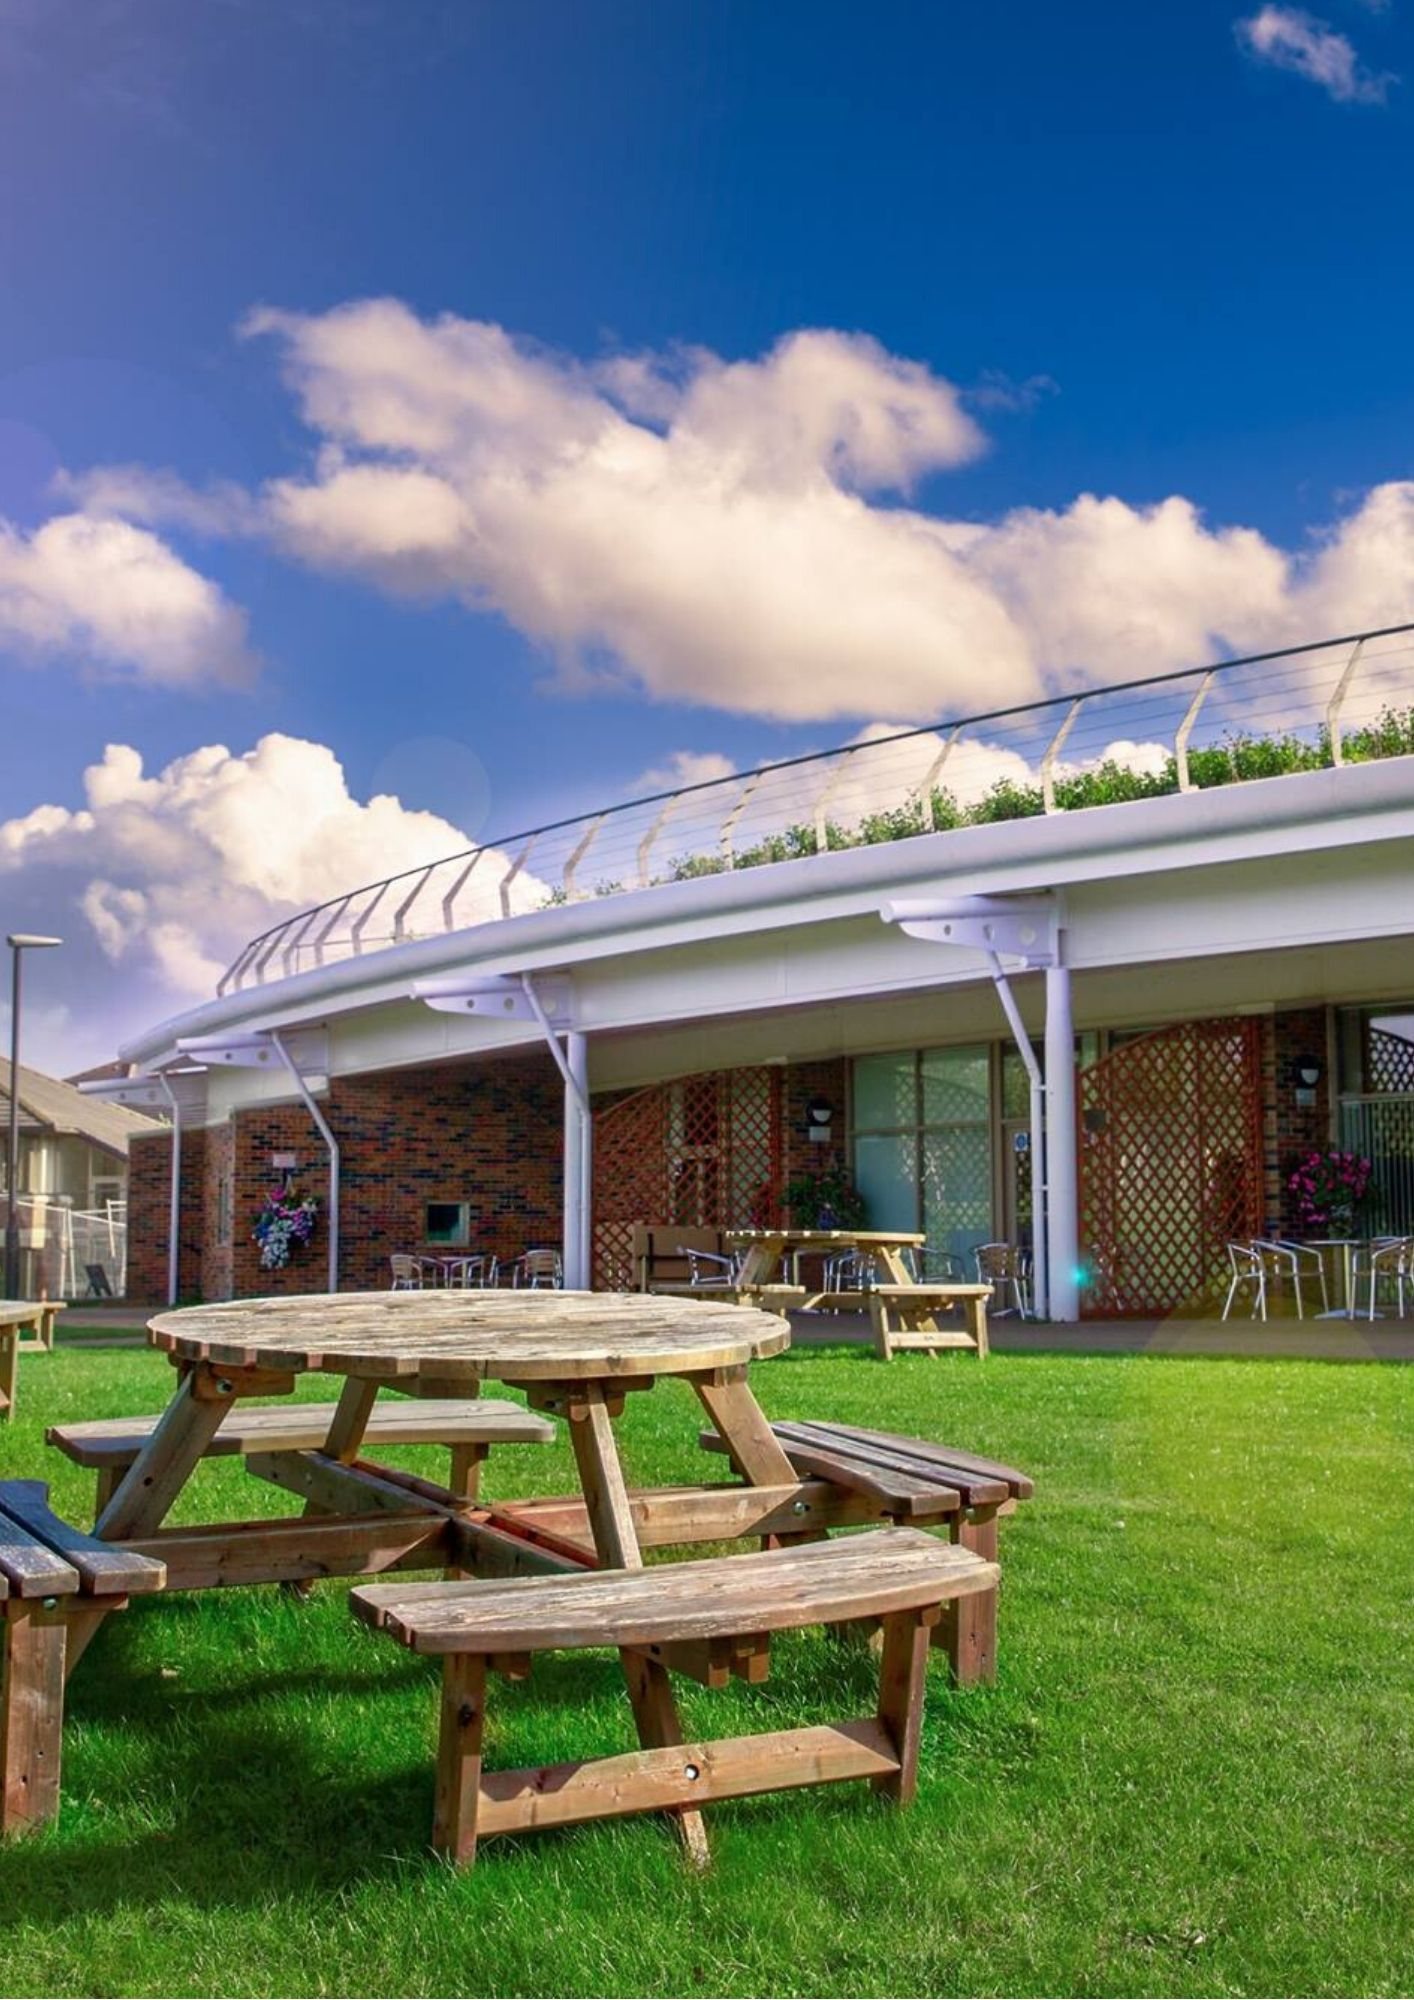
\includegraphics[width=\paperwidth,height=\paperheight,%
keepaspectratio]{Functional/tl.jpg}%
\vfill
}}}







